% Provenance (never printed): old premiere S material on subduction (Wadati-Benioff
% planes, density of the old lithosphere, slab pull, transformation of the slab at
% depth: blueschist and eclogite; anatomy of an active margin). Sections from
% figdata/grade-11/slab_sections.py (USGS ComCat M >= 6 1976-2025, PB2002 steps,
% Seton 2020 ages); plate speeds from plate_velocities.py (NNR-MORVEL56 RMS).
% Metamorphism is defined in g12.03, the volcanic arc in g12.04: named only here.
\chapter{俯冲带}\label{ch:g11:subduction-zones}

在西南太平洋的汤加群岛之下，地震
发生的深度远超其他任何地方。1976 至 2025 年间全球记录的七千次震级
6 或以上的地震中，最深的一次发生在
\qty{688}{km} 深处，本章的汤加剖面所含地震的震源可深至
约 \qty{671}{km}。在这样的深度，岩石温度很高，承受着巨大压力，
它本应像\omterm{def:g11:lithosphere-asthenosphere:lithosphere}{软流圈}那样缓慢流动，而不会断裂。然而它
断裂了。本章将说明那里有什么会断裂：一块冷的洋底\omterm{def:g11:subduction-zones:slab}{板片}，
正回沉入地幔之中。
% ledger: data:usgs-comcat (catalogue_maxdepth 688; tonga_maxdepth 670.8, slab_sections.py)

\begin{recall}
在汇聚型板块边界处，两个板块彼此相向运动；\omterm{def:g10:layered-ocean:thermocline}{深海}海沟
常位于其中一些边界处（第 1 册，七年级和八年级）。地震的震级
反映地震的大小，海底地震可引发海啸
（第 1 册，七年级）。一个板块相对另一个板块的速度
等于二者速度之差（见\cref{ch:g11:plate-motions}）。洋底
随年龄增长而下沉，约 6000 万年后其\omterm{def:g11:lithosphere-asthenosphere:lithosphere}{岩石圈}，
约 \qty{100}{km} 厚，密度大于其下方的\omterm{def:g11:lithosphere-asthenosphere:lithosphere}{软流圈}
（见\cref{ch:g11:ocean-ridges}）。地震波显示地幔中
约 \qty{670}{km} 深处有突变（见\cref{ch:g11:seismic-structure}）。变质岩
是在固态下发生转变的岩石（第 1 册，六年级）。
\end{recall}
% ledger: data:prem (670 km), ps77:depth-age

\section{海沟与倾斜地震带}

多数地震较浅。自 1976 年以来，震级为 6 或以上的地震中
仅约五分之一深于 \qty{70}{km}，十五分之一深于
\qty{300}{km}。下图显示深源地震的分布位置。
% values (slab_sections.py): frac_deeper_70 0.21, frac_deeper_300 0.069; data:usgs-comcat

\begin{omfigure}
\begin{tikzpicture}
\begin{axis}[ommap, width=\linewidth, xtick={-180,-90,...,180}, ytick={-60,0,60},
  legend style={font=\scriptsize, at={(0.5,-0.13)}, anchor=north, legend columns=3,
    /tikz/every even column/.append style={column sep=6pt}}]
\addplot[fill=omLithAlluv, draw=black!45, line width=0.2pt, forget plot] table {figdata/out/shared-geo-land.dat};
\addplot[black!70, line width=0.5pt, forget plot] table {figdata/out/shared-geo-school-subduction.dat};
\addplot[fill=black!70, draw=none, forget plot] table {figdata/out/shared-geo-school-teeth.dat};
% computed in figdata/grade-11/slab_sections.py; ledger: data:usgs-comcat, data:pb2002
\addplot[only marks, mark=*, mark size=0.55pt, black!45] table[x=lon, y=lat] {figdata/out/grade-11-slab_sections-world-shallow.dat};
\addplot[only marks, mark=*, mark size=0.8pt, omProp] table[x=lon, y=lat] {figdata/out/grade-11-slab_sections-world-mid.dat};
\addplot[only marks, mark=*, mark size=1.1pt, omThm] table[x=lon, y=lat] {figdata/out/grade-11-slab_sections-world-deep.dat};
\legend{{浅于 \qty{70}{km}}, {70 至 \qty{300}{km}}, {深于 \qty{300}{km}}}
\end{axis}
\end{tikzpicture}

{\small 震级 6.5 或以上的地震，1976--2025 年（共 2192 次），
按深度着色，图中标示海沟（黑线，三角形标在
上覆板块上）。中源和深源地震仅分布于部分海沟，
且总是位于上覆板块一侧。数据来源：USGS 地震目录；
板块边界取自 Bird（2003）；陆地数据来自 Natural Earth。}
\end{omfigure}
% values: world_n_m65 2192, world_deep_n 197 (slab_sections.py)

深源地震并非零散分布，它们沿着
西太平洋的海沟分布，从堪察加到日本、马里亚纳群岛、印度尼西亚和汤加，
以及南美洲西海岸的海沟；并且它们总是位于
海沟的一侧，即不下沉的那块板块之下。

\begin{definition}[俯冲；俯冲带]\label{def:g11:subduction-zones:subduction}
称\emph{俯冲}\index{俯冲}为\omterm{def:g11:ocean-ridges:oceanic-lithosphere}{大洋岩石圈}板块
俯入另一板块之下、回到地幔中的过程。
称\emph{俯冲带}\index{俯冲带}为俯冲发生的汇聚型板块边界，
地表以海沟为标志。
\end{definition}

\begin{definition}[和达–贝尼奥夫带]\label{def:g11:subduction-zones:benioff}
称\emph{和达–贝尼奥夫带}\index{和达–贝尼奥夫带}为倾斜的
地震带，始于海沟，并在上覆板块之下越来越深，
最深可达约 \qty{700}{km}。
\end{definition}
% ledger: frohlich87:wadati

\begin{history}[和达与贝尼奥夫]
1920 年代，主流地震学家认为地震只能
发生在地下最浅的几十千米之内：他们推断，深部地球
没有能力储存应变。日本地震学家和达清夫
曾与日本气象厅的密集台站网络合作，自 1928 年起
首次提出令人信服的证据，表明部分地震深达数百千米：
他研究的一次地震发生于 1927 年 1 月，深度为
\qty{420}{km}。1935 年，他发表了首张地震深度图，
以等高线绘出这些地震的深度，并注意到其加深的
地震带与活火山链平行。1949 年和 1954 年，美国地震学家
贝尼奥夫表明，安第斯山脉和
汤加–克马德克群岛之下，地震沿带分布，深度可达
约 \qty{700}{km}。这些地带于 1967 年首次被称为贝尼奥夫带；
而\omterm{def:g11:subduction-zones:benioff}{和达–贝尼奥夫带}这一名称兼顾了两人，
采纳的是日本地球物理学家上田诚也于 1971 年提出的建议。
\end{history}
% ledger: frohlich87:wadati

\begin{method}[读取地震剖面]\label{met:g11:subduction-zones:section}
\begin{enumerate}
  \item 选取一条与海沟垂直的直线，自海沟指向
        上覆板块一侧，并保留直线两侧一定宽度的
        条带内的地震。
  \item 将每次地震按其沿直线的距离（水平方向）
        及其深度（竖直向下）标出。
  \item 寻找倾斜的地震带，画出最能贴合它的
        直线。
  \item 利用直线上两点读出地震带的倾角
        （见下述命题）。
\end{enumerate}
\end{method}

\begin{omfigure}
\begin{tikzpicture}
\begin{axis}[omrecord, omdepth, name=tonga, width=0.5\linewidth, height=6.4cm,
  xmin=-150, xmax=900, ymin=0, ymax=720, xlabel={距海沟的距离（\unit{km}）},
  ylabel={深度（\unit{km}）}, title={\small 汤加}, clip=false]
% computed in figdata/grade-11/slab_sections.py; ledger: data:usgs-comcat, data:pb2002
\addplot[only marks, mark=*, mark size=1.2pt, black!65] table[x=x, y=depth] {figdata/out/grade-11-slab_sections-tonga.dat};
\addplot[omProp, line width=1pt, domain=135.7:761.6, samples=2] {-23.568 + 0.91068*x};
\addplot[only marks, mark=triangle*, mark size=3pt, omDef] coordinates {(0,0)};
\node[font=\scriptsize, anchor=south west, text=omDef] at (axis cs:10,8) {海沟};
\node[font=\scriptsize, anchor=west, text=omProp, align=left] at (axis cs:300,560) {倾角 \\\ang{42}};
\end{axis}
\begin{axis}[omrecord, omdepth, at={(tonga.east)}, anchor=west, xshift=0.3cm, width=0.5\linewidth, height=6.4cm,
  xmin=-150, xmax=900, ymin=0, ymax=720, xlabel={距海沟的距离（\unit{km}）},
  yticklabels={}, title={\small 安第斯山脉，南纬 \ang{21} 附近}, clip=false]
\addplot[only marks, mark=*, mark size=1.2pt, black!65] table[x=x, y=depth] {figdata/out/grade-11-slab_sections-andes.dat};
\addplot[omProp, line width=1pt, domain=253.0:900, samples=2] {-88.745 + 0.74613*x};
\addplot[only marks, mark=triangle*, mark size=3pt, omDef] coordinates {(0,0)};
\node[font=\scriptsize, anchor=south west, text=omDef] at (axis cs:10,8) {海沟};
\node[font=\scriptsize, anchor=west, text=omProp, align=left] at (axis cs:300,560) {倾角 \\\ang{37}};
\end{axis}
\end{tikzpicture}

{\small 垂直于两条海沟的地震剖面：
震级 6 级或以上、1976--2025 年间、距剖面线 \qty{150}{km} 以内的地震，
按其距海沟的距离（指向上覆板块一侧）及
深度绘制。橙色线为最能贴合
100 至 \qty{600}{km} 深度之间地震的直线。汤加下方的地震带
延伸至 \qty{670}{km} 以下。数据：USGS 地震目录；海沟位置取自 Bird（2003）。}
\end{omfigure}
% values (slab_sections.py): tonga_dip 42.3, fit -23.568 + 0.91068 x (77 events);
% andes_dip 36.7, fit -88.745 + 0.74613 x; trench points tonga (-173.31, -20.395),
% andes (-71.286, -21.01)

\begin{proposition}[由地震剖面求板片的倾角]\label{prop:g11:subduction-zones:dip}
若沿\omterm{def:g11:subduction-zones:benioff}{和达–贝尼奥夫带}所贴合直线上的两点
距海沟的水平距离分别为 $x_1 < x_2$，深度分别为 $z_1$ 与 $z_2$，
则其倾角 $\delta$（与水平面的夹角）满足
\[
  \tan \delta = \frac{z_2 - z_1}{x_2 - x_1}.
\]
\end{proposition}

\begin{proof}
两点及第二点正上方深度为 $z_1$ 的点
构成一个直角三角形，其水平边为 $x_2 - x_1$，竖直边为
$z_2 - z_1$，第一点处的角即为倾角。直角三角形中某锐角的正切
等于其对边与邻边之比。
\end{proof}

\begin{example}[汤加下方的倾角]\label{ex:g11:subduction-zones:dip}
汤加剖面上的直线在深 \qty{250}{km} 处经过距海沟
\qty{300}{km} 处，以及距海沟 \qty{700}{km} 处、深 \qty{614}{km} 处。因此
$\tan\delta = (614 - 250)/(700 - 300) = 364/400 = 0.91$，且
$\delta \approx \ang{42}$。在南纬 \ang{21}~附近的安第斯山脉下方，
用相同方法得到的倾角约为 \ang{37}。
\end{example}
% values: tonga line at 300 km 249.6, at 700 km 613.9 (slab_sections.py)

\omterm{def:g11:subduction-zones:benioff}{和达–贝尼奥夫带}勾勒出下沉的板块。浅源地震
发生在两板块彼此滑动之处，即靠近海沟的地方；较深的
地震则发生在下沉板块内部。

\section{为什么老的岩石圈会下沉}

\begin{definition}[板片]\label{def:g11:subduction-zones:slab}
称板块中已在\omterm{def:g11:subduction-zones:subduction}{俯冲带}处沉入地幔的部分为\emph{板片}\index{板片}，
即一层\omterm{def:g11:ocean-ridges:oceanic-lithosphere}{大洋岩石圈}，厚约百千米，
倾斜地位于上覆板块之下。
\end{definition}

下沉的是古老的洋底。由洋底的年龄可知，
抵达日本海沟（位于日本以东）的洋底约为 1.33 亿年，
抵达汤加海沟的洋底约为 9900 万年；即便是
抵达安第斯山脉的洋底（为最年轻的下沉洋底之一）
约为 4900 万年。这样古老的\omterm{def:g11:lithosphere-asthenosphere:lithosphere}{岩石圈}寒冷而厚重，
除较轻的地壳外，其密度比\omterm{def:g11:lithosphere-asthenosphere:lithosphere}{软流圈}大：一旦其一端
开始下沉，其自身重量便将其拉入。
% values (slab_sections.py): japan_age 133.1, tonga_age 98.8, andes_age 48.8 (median of the
% 1-degree cells 100-400 km seaward of the trench point); ledger data:b2-seafloor-age

\begin{definition}[板片拉力；洋脊推力]\label{def:g11:subduction-zones:slab-pull}
\emph{板片拉力}\index{板片拉力}是下沉的\omterm{def:g11:subduction-zones:slab}{板片}（密度大于周围地幔）
施加于所在板块其余部分的力，将其拉向
海沟。\emph{洋脊推力}\index{洋脊推力}是推动板块远离洋脊的力，
在洋脊处，年轻而炽热的\omterm{def:g11:lithosphere-asthenosphere:lithosphere}{岩石圈}高踞于隆起的洋脊之上，
并沿斜坡向下滑动。
\end{definition}

二者哪一个更重要？1975 年，唐纳德·福赛斯与上田诚也
根据板块的速度与形状推算出各力的强度：
下沉\omterm{def:g11:subduction-zones:slab}{板片}上的力控制着大洋板块的速度，
且强度约为其他任何力的十倍。当今板块
速度清楚地证明了这一点。
% ledger: fu75:slab-pull

\begin{omfigure}
\begin{tikzpicture}
\begin{axis}[omrecord, ybar, bar width=9pt, width=0.86\linewidth, height=5.6cm,
  ymin=0, ymax=85, xmin=-0.7, xmax=12.7, bar shift=0pt, ylabel={平均速度（\unit{mm}/年）},
  xtick={0,...,12}, xticklabel style={rotate=50, anchor=east, font=\scriptsize},
  xticklabels={科科斯,纳斯卡,太平洋,澳大利亚,菲律宾海,阿拉伯,索马里,
    努比亚,欧亚,北美,南极,加勒比,南美},
  ymajorgrids, xmajorgrids=false]
% computed in figdata/grade-11/slab_sections.py from plate_velocities.POLES (nnr56:rms)
\addplot[fill=omProp, draw=omProp!70!black] table[x=idx, y expr=\thisrow{slab}*\thisrow{rms}] {figdata/out/grade-11-slab_sections-speeds.dat};
\addplot[fill=omDef!35, draw=omDef] table[x=idx, y expr=(1-\thisrow{slab})*\thisrow{rms}] {figdata/out/grade-11-slab_sections-speeds.dat};
\node[font=\scriptsize, text=omProp!80!black, anchor=south] at (axis cs:2,76) {板片悬挂于板块上};
\node[font=\scriptsize, text=omDef, anchor=south] at (axis cs:9,50) {无长板片};
\end{axis}
\end{tikzpicture}

{\small 十三个大板块的平均速度（对每个板块取方均根，
以\omterm{def:g11:lithosphere-asthenosphere:lithosphere}{岩石圈}整体不转动的参考系计算）。
橙色：沿较长边界有下沉\omterm{def:g11:subduction-zones:slab}{板片}悬挂的板块；
蓝色：无此类\omterm{def:g11:subduction-zones:slab}{板片}的板块。印度未列入：其北缘为
碰撞带。数据来自 NNR-MORVEL56（Argus、Gordon 和 DeMets，
2011）。}
\end{omfigure}
% ledger: nnr56:rms; the bars of a class are drawn at 0 for the other (two series on one axis)

\begin{proposition}[与板片相连的板块运动得快]\label{prop:g11:subduction-zones:fast}
长\omterm{def:g11:subduction-zones:slab}{板片}悬挂于其上的五个大板块（科科斯、纳斯卡、太平洋、
澳大利亚、菲律宾海）平均速度约为每年 \qty{65}{mm}；其余
八个无\omterm{def:g11:subduction-zones:slab}{板片}的板块约为每年 \qty{24}{mm}，慢近三倍。
第一组中每个板块都快于第二组中的任何板块。
\end{proposition}
% values: rms_slab_mean 65.2, rms_noslab_mean 23.9 (plate_velocities.py); India left out
% (its northern edge is a collision)

\begin{proof}
由已发表的平均速度，有\omterm{def:g11:subduction-zones:slab}{板片}的板块给出
$(74.6 + 70.0 + 65.5 + 63.1 + 52.6)/5 \approx 65.2$，其余板块则为
$(47.6 + 31.0 + 29.2 + 22.8 + 19.8 + 15.2 + 14.9 + 10.6)/8 \approx 23.9$
（毫米每年）；有\omterm{def:g11:subduction-zones:slab}{板片}的板块中最慢的菲律宾海板块，其速度为
52.6，仍快于其余板块中最快的阿拉伯板块（47.6）。
\end{proof}
% ledger: nnr56:rms

\section{板片在深部的转变}

\omterm{def:g11:subduction-zones:slab}{板片}下沉时，由玄武岩和\omterm{def:g11:ocean-ridges:gabbro}{辉长岩}构成的地壳被埋得越来越深，
同时保持低温，因为\omterm{def:g11:subduction-zones:slab}{板片}下沉的速度快于热量传入
其内部的速度。地壳岩石在不熔化的情况下改变其矿物组成：它们
发生变质（见\cref{ch:g12:metamorphic-rocks}）。两种岩石标示了这条路径。

\begin{definition}[蓝片岩；榴辉岩]\label{def:g11:subduction-zones:eclogite}
\emph{蓝片岩}\index{蓝片岩}是一种变质岩，由大洋地壳中的玄武岩
在保持相对低温的同时被埋至高压环境中形成；
它因含矿物蓝闪石而呈蓝色。\emph{榴辉岩}\index{榴辉岩}
是玄武岩和\omterm{def:g11:ocean-ridges:gabbro}{辉长岩}在地幔深度沿\omterm{def:g11:subduction-zones:subduction}{俯冲带}转变而成的致密变质岩：
它的化学组成与原岩相同，但由
红色石榴石与绿色辉石组成。
\end{definition}
% ledger: photo:g11-blueschist, photo:g11-eclogite

\begin{omfigure}
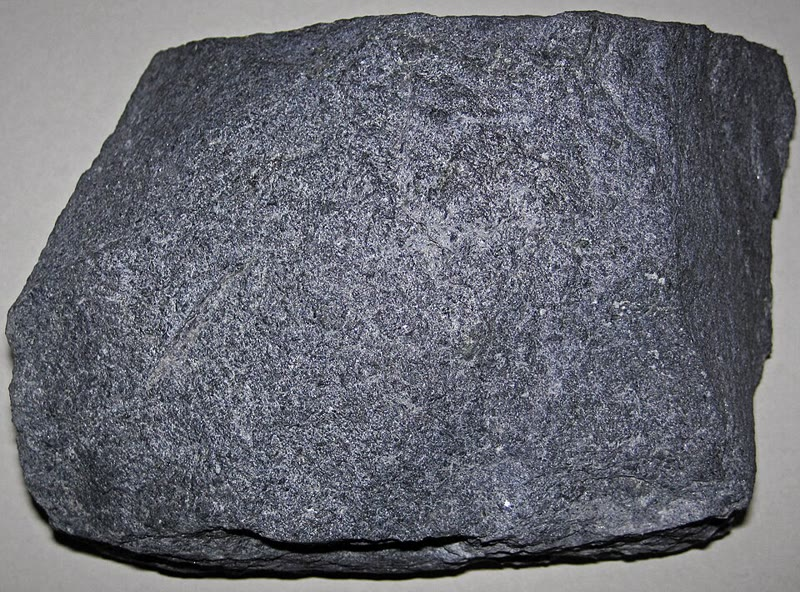
\includegraphics[height=4.4cm]{images/book2/g11-stjohn-blueschist.jpg}\hspace{0.03\linewidth}%
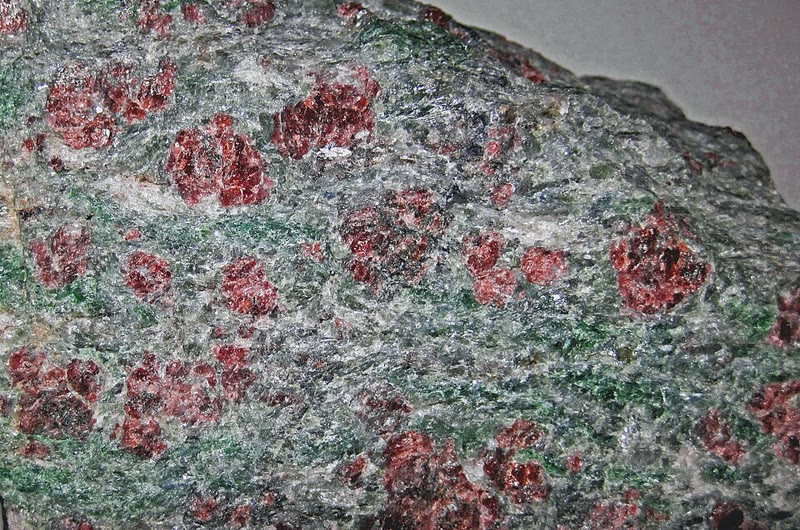
\includegraphics[height=4.4cm]{images/book2/g11-stjohn-eclogite.jpg}

{\small 左：来自加利福尼亚州圣卡塔利纳岛的\omterm{def:g11:subduction-zones:eclogite}{蓝片岩}，曾是
\omterm{def:g11:subduction-zones:subduction}{俯冲带}中被埋藏的大洋地壳。右：来自挪威的\omterm{def:g11:subduction-zones:eclogite}{榴辉岩}，红色
石榴石嵌于绿色辉石中。照片：James St.~John（CC~BY~2.0）。}
\end{omfigure}
% ledger: photo:g11-blueschist, photo:g11-eclogite

\omterm{def:g11:subduction-zones:eclogite}{榴辉岩}比玄武岩致密，甚至比地幔中的\omterm{def:g11:ocean-ridges:peridotite}{橄榄岩}
约致密 \qty{6}{\percent}。一旦其地壳变为\omterm{def:g11:subduction-zones:eclogite}{榴辉岩}，
\omterm{def:g11:subduction-zones:slab}{板片}便不再在顶部承载轻质层：整个\omterm{def:g11:subduction-zones:slab}{板片}
比周围地幔更致密，拉力也更大。这类岩石经后来的构造运动被带回
地表，是少数能直接见证
\omterm{def:g11:subduction-zones:subduction}{俯冲带}中数十千米深处所发生之事的直接证据。
% ledger: hacker03:eclogite, photo:g11-eclogite

\begin{omfigure}
\begin{tikzpicture}[font=\footnotesize, scale=0.85]
  % subduction zone, a drawing, not to scale: slab top flat to x = -1, then bends to a 42-degree dip
  % coordinates computed once by a small script (scratch, not kept): slab top flat to x=-1, arc R=3 to a 42-degree dip
  \fill[omProp!10] (-7,-1.4) rectangle (7,-6.0);
  \fill[omSea!45] (-7,0) -- (-1,0) -- (1.6,0.8) -- (-7,0.8) -- cycle;
  \fill[lith peridotite] (-7.000,0.000) -- (-6.644,0.000) -- (-6.289,0.000) -- (-5.933,0.000) -- (-5.578,0.000) -- (-5.222,0.000) -- (-4.867,0.000) -- (-4.511,0.000) -- (-4.156,0.000) -- (-3.800,0.000) -- (-3.445,0.000) -- (-3.089,0.000) -- (-2.734,0.000) -- (-2.378,0.000) -- (-2.023,0.000) -- (-1.667,0.000) -- (-1.312,0.000) -- (-0.956,-0.000) -- (-0.602,-0.027) -- (-0.253,-0.094) -- (0.085,-0.203) -- (0.408,-0.351) -- (0.712,-0.536) -- (0.991,-0.756) -- (1.255,-0.994) -- (1.519,-1.232) -- (1.784,-1.470) -- (2.048,-1.707) -- (2.312,-1.945) -- (2.576,-2.183) -- (2.840,-2.421) -- (3.105,-2.659) -- (3.369,-2.897) -- (3.633,-3.135) -- (3.897,-3.373) -- (4.161,-3.611) -- (4.426,-3.848) -- (4.690,-4.086) -- (4.954,-4.324) -- (5.218,-4.562) -- (5.483,-4.800) -- (4.546,-5.840) -- (4.282,-5.603) -- (4.017,-5.365) -- (3.753,-5.127) -- (3.489,-4.889) -- (3.225,-4.651) -- (2.961,-4.413) -- (2.696,-4.175) -- (2.432,-3.937) -- (2.168,-3.699) -- (1.904,-3.461) -- (1.639,-3.224) -- (1.375,-2.986) -- (1.111,-2.748) -- (0.847,-2.510) -- (0.583,-2.272) -- (0.318,-2.034) -- (0.062,-1.803) -- (-0.087,-1.686) -- (-0.249,-1.587) -- (-0.421,-1.508) -- (-0.602,-1.450) -- (-0.788,-1.414) -- (-0.977,-1.400) -- (-1.312,-1.400) -- (-1.667,-1.400) -- (-2.023,-1.400) -- (-2.378,-1.400) -- (-2.734,-1.400) -- (-3.089,-1.400) -- (-3.445,-1.400) -- (-3.800,-1.400) -- (-4.156,-1.400) -- (-4.511,-1.400) -- (-4.867,-1.400) -- (-5.222,-1.400) -- (-5.578,-1.400) -- (-5.933,-1.400) -- (-6.289,-1.400) -- (-6.644,-1.400) -- (-7.000,-1.400) -- cycle;
  \fill[lith basalt] (-7.000,0.000) -- (-6.644,0.000) -- (-6.289,0.000) -- (-5.933,0.000) -- (-5.578,0.000) -- (-5.222,0.000) -- (-4.867,0.000) -- (-4.511,0.000) -- (-4.156,0.000) -- (-3.800,0.000) -- (-3.445,0.000) -- (-3.089,0.000) -- (-2.734,0.000) -- (-2.378,0.000) -- (-2.023,0.000) -- (-1.667,0.000) -- (-1.312,0.000) -- (-0.956,-0.000) -- (-0.602,-0.027) -- (-0.253,-0.094) -- (0.085,-0.203) -- (0.408,-0.351) -- (0.712,-0.536) -- (0.991,-0.756) -- (1.255,-0.994) -- (1.519,-1.232) -- (1.784,-1.470) -- (2.048,-1.707) -- (2.312,-1.945) -- (2.576,-2.183) -- (2.840,-2.421) -- (3.105,-2.659) -- (3.369,-2.897) -- (3.633,-3.135) -- (3.897,-3.373) -- (4.161,-3.611) -- (4.426,-3.848) -- (4.690,-4.086) -- (4.954,-4.324) -- (5.218,-4.562) -- (5.483,-4.800) -- (5.282,-5.023) -- (5.018,-4.785) -- (4.753,-4.547) -- (4.489,-4.309) -- (4.225,-4.071) -- (3.961,-3.833) -- (3.697,-3.596) -- (3.432,-3.358) -- (3.168,-3.120) -- (2.904,-2.882) -- (2.640,-2.644) -- (2.376,-2.406) -- (2.111,-2.168) -- (1.847,-1.930) -- (1.583,-1.692) -- (1.319,-1.455) -- (1.054,-1.217) -- (0.792,-0.980) -- (0.541,-0.783) -- (0.268,-0.616) -- (-0.023,-0.483) -- (-0.328,-0.385) -- (-0.642,-0.324) -- (-0.960,-0.300) -- (-1.312,-0.300) -- (-1.667,-0.300) -- (-2.023,-0.300) -- (-2.378,-0.300) -- (-2.734,-0.300) -- (-3.089,-0.300) -- (-3.445,-0.300) -- (-3.800,-0.300) -- (-4.156,-0.300) -- (-4.511,-0.300) -- (-4.867,-0.300) -- (-5.222,-0.300) -- (-5.578,-0.300) -- (-5.933,-0.300) -- (-6.289,-0.300) -- (-6.644,-0.300) -- (-7.000,-0.300) -- cycle;
  \fill[blue!30] (2.484,-2.100) -- (2.604,-2.208) -- (2.725,-2.317) -- (2.845,-2.425) -- (2.965,-2.533) -- (3.085,-2.642) -- (3.206,-2.750) -- (3.326,-2.858) -- (3.446,-2.967) -- (3.567,-3.075) -- (3.687,-3.183) -- (3.807,-3.292) -- (3.928,-3.400) -- (3.727,-3.623) -- (3.607,-3.515) -- (3.486,-3.406) -- (3.366,-3.298) -- (3.246,-3.190) -- (3.125,-3.081) -- (3.005,-2.973) -- (2.885,-2.865) -- (2.764,-2.756) -- (2.644,-2.648) -- (2.524,-2.540) -- (2.403,-2.431) -- (2.283,-2.323) -- cycle;
  \fill[lith eclogite] (3.928,-3.400) -- (4.057,-3.517) -- (4.187,-3.633) -- (4.316,-3.750) -- (4.446,-3.867) -- (4.576,-3.983) -- (4.705,-4.100) -- (4.835,-4.217) -- (4.964,-4.333) -- (5.094,-4.450) -- (5.223,-4.567) -- (5.353,-4.683) -- (5.483,-4.800) -- (5.282,-5.023) -- (5.152,-4.906) -- (5.023,-4.790) -- (4.893,-4.673) -- (4.764,-4.556) -- (4.634,-4.440) -- (4.504,-4.323) -- (4.375,-4.206) -- (4.245,-4.090) -- (4.116,-3.973) -- (3.986,-3.856) -- (3.857,-3.740) -- (3.727,-3.623) -- cycle;
  \draw[black!60] (-7.000,0.000) -- (-6.644,0.000) -- (-6.289,0.000) -- (-5.933,0.000) -- (-5.578,0.000) -- (-5.222,0.000) -- (-4.867,0.000) -- (-4.511,0.000) -- (-4.156,0.000) -- (-3.800,0.000) -- (-3.445,0.000) -- (-3.089,0.000) -- (-2.734,0.000) -- (-2.378,0.000) -- (-2.023,0.000) -- (-1.667,0.000) -- (-1.312,0.000) -- (-0.956,-0.000) -- (-0.602,-0.027) -- (-0.253,-0.094) -- (0.085,-0.203) -- (0.408,-0.351) -- (0.712,-0.536) -- (0.991,-0.756) -- (1.255,-0.994) -- (1.519,-1.232) -- (1.784,-1.470) -- (2.048,-1.707) -- (2.312,-1.945) -- (2.576,-2.183) -- (2.840,-2.421) -- (3.105,-2.659) -- (3.369,-2.897) -- (3.633,-3.135) -- (3.897,-3.373) -- (4.161,-3.611) -- (4.426,-3.848) -- (4.690,-4.086) -- (4.954,-4.324) -- (5.218,-4.562) -- (5.483,-4.800);
  \draw[black!60] (-7.000,-1.400) -- (-6.644,-1.400) -- (-6.289,-1.400) -- (-5.933,-1.400) -- (-5.578,-1.400) -- (-5.222,-1.400) -- (-4.867,-1.400) -- (-4.511,-1.400) -- (-4.156,-1.400) -- (-3.800,-1.400) -- (-3.445,-1.400) -- (-3.089,-1.400) -- (-2.734,-1.400) -- (-2.378,-1.400) -- (-2.023,-1.400) -- (-1.667,-1.400) -- (-1.312,-1.400) -- (-0.977,-1.400) -- (-0.788,-1.414) -- (-0.602,-1.450) -- (-0.421,-1.508) -- (-0.249,-1.587) -- (-0.087,-1.686) -- (0.062,-1.803) -- (0.318,-2.034) -- (0.583,-2.272) -- (0.847,-2.510) -- (1.111,-2.748) -- (1.375,-2.986) -- (1.639,-3.224) -- (1.904,-3.461) -- (2.168,-3.699) -- (2.432,-3.937) -- (2.696,-4.175) -- (2.961,-4.413) -- (3.225,-4.651) -- (3.489,-4.889) -- (3.753,-5.127) -- (4.017,-5.365) -- (4.282,-5.603) -- (4.546,-5.840);
  \draw[black!60] (5.483,-4.800) -- (4.546,-5.840);
  \fill[omLithGranite!55] (-1.000,0.000) -- (1.600,0.800) -- (7.000,0.800) -- (7.000,-1.600) -- (1.929,-1.600) -- (1.801,-1.485) -- (1.673,-1.370) -- (1.545,-1.255) -- (1.417,-1.140) -- (1.290,-1.025) -- (1.162,-0.910) -- (1.034,-0.795) -- (0.904,-0.682) -- (0.768,-0.577) -- (0.627,-0.479) -- (0.480,-0.390) -- (0.328,-0.310) -- (0.172,-0.238) -- (0.011,-0.176) -- (-0.152,-0.122) -- (-0.318,-0.078) -- (-0.487,-0.044) -- (-0.657,-0.020) -- (-0.828,-0.005) -- (-1.000,0.000) -- cycle;
  \fill[omLithAlluv] (-1.000,0.000) -- (0.550,0.470) -- (0.926,-0.700) -- (0.761,-0.571) -- (0.588,-0.455) -- (0.407,-0.350) -- (0.219,-0.259) -- (0.025,-0.180) -- (-0.174,-0.116) -- (-0.377,-0.065) -- (-0.583,-0.029) -- (-0.791,-0.007) -- (-1.000,0.000) -- cycle;
  \draw[black!60] (-1.000,0.000) -- (1.600,0.800) -- (7.000,0.800) -- (7.000,-1.600) -- (1.929,-1.600) -- (1.801,-1.485) -- (1.673,-1.370) -- (1.545,-1.255) -- (1.417,-1.140) -- (1.290,-1.025) -- (1.162,-0.910) -- (1.034,-0.795) -- (0.904,-0.682) -- (0.768,-0.577) -- (0.627,-0.479) -- (0.480,-0.390) -- (0.328,-0.310) -- (0.172,-0.238) -- (0.011,-0.176) -- (-0.152,-0.122) -- (-0.318,-0.078) -- (-0.487,-0.044) -- (-0.657,-0.020) -- (-0.828,-0.005) -- (-1.000,0.000);
  \draw[omThm!75, densely dashed, line width=0.7pt] (-7.000,-1.150) -- (-6.648,-1.150) -- (-6.296,-1.150) -- (-5.945,-1.150) -- (-5.593,-1.150) -- (-5.241,-1.150) -- (-4.889,-1.150) -- (-4.538,-1.150) -- (-4.186,-1.150) -- (-3.834,-1.150) -- (-3.482,-1.150) -- (-3.130,-1.150) -- (-2.779,-1.150) -- (-2.427,-1.150) -- (-2.075,-1.150) -- (-1.723,-1.150) -- (-1.372,-1.150) -- (-1.020,-1.150) -- (-0.796,-1.161) -- (-0.582,-1.198) -- (-0.374,-1.259) -- (-0.175,-1.344) -- (0.013,-1.452) -- (0.187,-1.581) -- (0.419,-1.788) -- (0.680,-2.023) -- (0.942,-2.259) -- (1.203,-2.494) -- (1.465,-2.730) -- (1.726,-2.965) -- (1.987,-3.200) -- (2.249,-3.436) -- (2.510,-3.671) -- (2.772,-3.907) -- (3.033,-4.142) -- (3.294,-4.377) -- (3.556,-4.613) -- (3.817,-4.848) -- (4.079,-5.083) -- (4.340,-5.319) -- (4.602,-5.554) -- (5.103,-4.997) -- (5.045,-4.944) -- (4.987,-4.892) -- (4.929,-4.839) -- (4.870,-4.787) -- (4.812,-4.734) -- (4.754,-4.682) -- (4.695,-4.629) -- (4.637,-4.577) -- (4.579,-4.524) -- (4.520,-4.472) -- (4.462,-4.419) -- (4.404,-4.367) -- (4.346,-4.315) -- (4.287,-4.262) -- (4.229,-4.210) -- (4.171,-4.157) -- (4.112,-4.105) -- (4.054,-4.052) -- (3.996,-4.000) -- (3.937,-3.947) -- (3.879,-3.895) -- (3.821,-3.842) -- (3.763,-3.790) -- (3.704,-3.737) -- (3.646,-3.685) -- (3.588,-3.632) -- (3.529,-3.580) -- (3.471,-3.527) -- (3.413,-3.475) -- (3.355,-3.422) -- (3.296,-3.370) -- (3.238,-3.317) -- (3.180,-3.265) -- (3.121,-3.212) -- (3.063,-3.160) -- (3.005,-3.107) -- (2.946,-3.055) -- (2.888,-3.002) -- (2.830,-2.950) -- (2.772,-2.897) -- (7.000,-2.897);
  \foreach \p in {(-0.72,-0.22),(-0.46,-0.36),(-0.18,-0.37),(0.05,-0.55),(0.29,-0.67),(0.63,-0.66),(0.87,-0.82),(0.91,-1.23),(1.27,-1.29),(1.50,-1.49),(1.55,-1.89),(1.90,-1.96),(2.04,-2.25),(2.35,-2.36),(2.54,-2.61),(2.88,-2.69),(2.99,-3.02),(3.16,-3.28),(3.47,-3.40),(3.65,-3.66),(3.89,-3.84),(4.26,-3.89),(4.32,-4.27),(4.59,-4.43),(4.88,-4.56),(5.17,-4.70)} \fill[black] \p circle (1.3pt);
  % volcanic arc above the slab, back-arc stretched
  \fill[black!70] (3.35,0.8) -- (3.7,1.4) -- (4.05,0.8) -- cycle;
  \draw[black!45, dashed] (5.2,0.8) -- (5.2,-1.6); \draw[black!45, dashed] (6.6,0.8) -- (6.6,-1.6);
  \draw[{Stealth[length=4pt]}-{Stealth[length=4pt]}, black!70] (5.35,-0.7) -- (6.45,-0.7);
  % motion arrows
  \draw[-{Stealth[length=5pt]}, line width=1pt] (-5.6,0.4) -- (-3.6,0.4);
  \draw[-{Stealth[length=5pt]}, line width=1pt] (1.77,-4.01) -- (2.88,-5.01);
  % labels
  \draw[black!60] (-1.0,0.02) -- (-1.8,1.05);
  \node[anchor=south] at (-1.8,1.05) {海沟};
  \draw[black!60] (0.1,0.12) -- (0.5,1.05);
  \node[anchor=south, align=center] at (0.6,1.05) {沉积物 \\被刮下};
  \node[anchor=south] at (2.35,0.85) {弧前};
  \node[anchor=south] at (3.7,1.4) {火山弧};
  \node[anchor=south] at (5.9,0.85) {弧后};
  \node[anchor=south] at (-5.4,0.82) {大洋底向海沟移动};
  \draw[black!60] (-7.0,-0.15) -- (-7.25,-0.15);
  \node[anchor=east] at (-7.25,-0.15) {大洋地壳};
  \draw[black!60] (-7.0,-0.85) -- (-7.25,-0.85);
  \node[anchor=east, align=right] at (-7.25,-0.85) {岩石圈地幔 \\部分};
  \node at (-3.5,-3.6) {软流圈};
  \node[rotate=-42] at (3.98,-4.46) {板片};
  \draw[black!60] (3.35,-2.65) -- (4.3,-2.35);
  \node[anchor=west] at (4.3,-2.35) {蓝片岩};
  \draw[black!60] (5.1,-4.3) -- (5.75,-4.6);
  \node[anchor=west] at (5.75,-4.6) {榴辉岩};
  \node[anchor=north east, text=omThm!80!black, align=right] at (7,-2.95) {等温 \\线};
  \fill[black] (-6.8,-5.55) circle (1.3pt);
  \node[anchor=west] at (-6.65,-5.55) {地震};
\end{tikzpicture}

{\small \omterm{def:g11:subduction-zones:subduction}{俯冲带}示意图（非按比例绘制）。较老的\omterm{def:g11:ocean-ridges:oceanic-lithosphere}{大洋岩石圈}
在海沟处弯曲向下，\omterm{def:g11:subduction-zones:subduction}{俯冲}到上覆板块之下。刮落于其表面的沉积物
堆积在上覆板块边缘；地震沿下沉\omterm{def:g11:subduction-zones:slab}{板片}分布；地壳先转变为\omterm{def:g11:subduction-zones:eclogite}{蓝片岩}，
继而转变为\omterm{def:g11:subduction-zones:eclogite}{榴辉岩}。\omterm{def:g11:subduction-zones:slab}{板片}比周围地幔更冷，等温线
沿\omterm{def:g11:subduction-zones:slab}{板片}向下被拖曳。
一列火山即火山弧，
位于\omterm{def:g11:subduction-zones:slab}{板片}上方。}
\end{omfigure}
% volcanic arc above the slab: told only, defined and sourced in g12.04

\section{俯冲带的结构}

从大洋到大陆，或到下一个大洋，
\omterm{def:g11:subduction-zones:subduction}{俯冲带}总是由相同的几部分组成。

\begin{itemize}
  \item \emph{海沟}：下沉板块弯曲向下的地方，
        是大洋中最深的地方。
  \item \emph{弧前}：位于海沟与火山线之间，其
        前缘是由下沉板块刮落的沉积物堆积而成；其下方
        两板块沿板块边界相互错动，
        这是一条倾角平缓的断层，巨大地震就发生在其上，例如
        2011 年日本近海的那次（见下文例）。
  \item \emph{火山弧}：与海沟平行的一列火山，
        位于岛屿（汤加、马里亚纳群岛、日本）或大陆（安第斯山脉）上；
        其成因将在\cref{ch:g12:subduction-magmatism}中讨论。
  \item 某些火山弧之后存在\emph{弧后}区域，其上覆板块
        被拉伸；在汤加，弧后正被拉开。
\end{itemize}
% ledger: bevis95:tonga (back-arc extension at Tonga); usgs:tohoku (largest earthquakes on the
% plate boundary: example below)

在汤加，弧后的拉伸使火山弧本身向
太平洋板块方向移动，卫星定位已证实这一点。汤加海沟两侧的汇聚速率
因此大于任一板块自身的速度：据 PB2002 模型，
在南纬 \ang{20} 附近，约为每年 \qty{17}{cm}。
% values: tonga_rate 168.0 (mean of the PB2002 TO/PA steps within 100 km of the profile);
% PB2002 steps along Tonga: 104 to 237 mm/yr; ledger data:pb2002, bevis95:tonga

\begin{example}[2011 年东北地震]\label{ex:g11:subduction-zones:tohoku}
2011 年 3 月 11 日，一场震级为 9.1 的地震袭击了日本本州东北
海岸外海。地震发生在约 \qty{25}{km} 深处，就在板块
边界上，太平洋板块以约每年 \qty{83}{mm} 的速度
向西运动（相对于承载日本北部的板块），在日本海沟
处\omterm{def:g11:subduction-zones:subduction}{俯冲}到其下方。断层两侧相互错动，最大错动量达 50 至
\qty{60}{m}，错动区域约 \qty{400}{km} 长、
\qty{150}{km} 宽。上方的海底随之移动，并引发了海啸，
其在海岸上爬升至 \qty{38}{m} 高，造成至少 \num{15703} 人
遇难，\num{4647} 人失踪。同一海岸此前曾遭受
该\omterm{def:g11:subduction-zones:subduction}{俯冲带}引发的海啸，分别发生于 1611 年、1896 年和 1933 年，
也许在 869 年还曾遭受过一次与 2011 年同等规模的海啸。
\end{example}
% ledger: usgs:tohoku

\begin{omfigure}
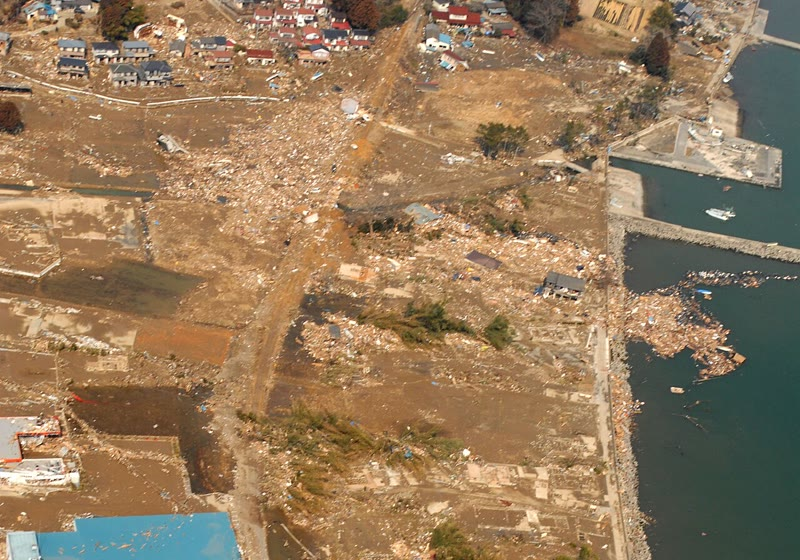
\includegraphics[width=0.78\linewidth]{images/book2/g11-usn-tsunami-kesennuma.jpg}

{\small 气仙沼渔港，位于日本东北海岸，拍摄于
2011 年 3 月 11 日海啸两天后。照片：Dylan McCord, U.S. Navy
（公有领域）。}
\end{omfigure}
% ledger: photo:g11-tsunami

\section{练习}

\begin{exercise}[$\star$]\label{exo:g11:subduction-zones:1}
给出\omterm{def:g11:subduction-zones:subduction}{俯冲}与\omterm{def:g11:subduction-zones:subduction}{俯冲带}的定义。在\omterm{def:g11:subduction-zones:subduction}{俯冲带}处下沉的是哪一类
\omterm{def:g11:lithosphere-asthenosphere:lithosphere}{岩石圈}，并说明为什么是这一类？
\end{exercise}

\begin{exercise}[$\star$]\label{exo:g11:subduction-zones:2}
利用按深度划分的世界地震图：（1）指出三个震源深度
超过 \qty{300}{km} 的地区；（2）深源地震位于海沟的哪一侧？
（3）沿大西洋中脊，地震的深度
如何？
\end{exercise}

\begin{exercise}[$\star$]\label{exo:g11:subduction-zones:3}
目录中共收录 \num{7031} 次震级为 6 或以上的地震，其中
\qty{21}{\percent} 的地震深度超过 \qty{70}{km}，\qty{6.9}{\percent}
的地震深度超过 \qty{300}{km}。各为多少次地震？
\end{exercise}

\begin{exercise}[$\star$]\label{exo:g11:subduction-zones:4}
给出\omterm{def:g11:subduction-zones:eclogite}{蓝片岩}与\omterm{def:g11:subduction-zones:eclogite}{榴辉岩}的定义。二者与\omterm{def:g11:ocean-ridges:oceanic-lithosphere}{洋壳}玄武岩
有哪些共同点？又有哪些不同？
\end{exercise}

\begin{exercise}[$\star$]\label{exo:g11:subduction-zones:5}
按顺序列出\omterm{def:g11:subduction-zones:subduction}{俯冲带}的各组成部分，
从朝向海沟运动的洋底直到弧后，
并用一句话说明每一部分中发生了什么。
\end{exercise}

\begin{exercise}[$\star\star$]\label{exo:g11:subduction-zones:6}
在安第斯剖面上，沿地震分布的那条线经过距海沟
\qty{300}{km} 处、深 \qty{135}{km} 的点，以及距海沟
\qty{800}{km} 处、深 \qty{508}{km} 的点。求\omterm{def:g11:subduction-zones:slab}{板片}的倾角。
\end{exercise}

\begin{exercise}[$\star\star$]\label{exo:g11:subduction-zones:7}
一块直线形\omterm{def:g11:subduction-zones:slab}{板片}从海沟处向下延伸，倾角为 \ang{45}。（1）
距海沟 \qty{300}{km} 处的\omterm{def:g11:subduction-zones:slab}{板片}深度是多少？（2）它在距海沟
多远处深度达到 \qty{670}{km}？（3）海沟与
\qty{670}{km} 深度之间的\omterm{def:g11:subduction-zones:slab}{板片}长度为多少？
\end{exercise}

\begin{exercise}[$\star\star$]\label{exo:g11:subduction-zones:8}
各板块的平均速度（单位为毫米每年）如下：科科斯 74.6、纳斯卡
70.0、太平洋 65.5、澳大利亚 63.1、菲律宾海 52.6（有\omterm{def:g11:subduction-zones:slab}{板片}）；阿拉伯
47.6、索马里 31.0、努比亚 29.2、欧亚 22.8、北美 19.8、南极
15.2、加勒比 14.9、南美 10.6（无\omterm{def:g11:subduction-zones:slab}{板片}）。（1）计算各组的平均值
及其比值。（2）这对驱动板块运动的作用力
说明了什么？
\end{exercise}

\begin{exercise}[$\star\star$]\label{exo:g11:subduction-zones:9}
2011 年，日本近海的断层最多错动了 50 至 \qty{60}{m}。太平洋板块
每年以 \qty{83}{mm} 的速度逼近。（1）错动 \qty{50}{m}、再错动 \qty{60}{m}，
分别相当于多少年的板块运动？（2）将其与自 869 年以来的时间相比，
869 年可能曾发生过同等规模的更早地震。
\end{exercise}

\begin{exercise}[$\star\star$]\label{exo:g11:subduction-zones:10}
抵达日本海沟的洋底年龄约为 13300 万年，
抵达汤加的约为 9900 万年，抵达安第斯山脉的约为 4900 万年。（1）
利用\cref{ch:g11:ocean-ridges}中的规律（$2500 + 350\sqrt{t}$，
适用于 $t \le 70$；超过时为 $6400 - 3200\,e^{-t/62.8}$），求各处的深度。（2）
哪一处的\omterm{def:g11:lithosphere-asthenosphere:lithosphere}{岩石圈}最冷、最致密？
\end{exercise}

\begin{exercise}[$\star\star$]\label{exo:g11:subduction-zones:11}
\omterm{def:g11:ocean-ridges:oceanic-lithosphere}{洋壳}玄武岩的密度约为 \qty{2900}{kg/m^3}，
\omterm{def:g11:subduction-zones:slab}{板片}周围地幔的密度为 \qty{3380}{kg/m^3}，\omterm{def:g11:subduction-zones:eclogite}{榴辉岩}的密度比地幔大
\qty{6}{\percent}。（1）求\omterm{def:g11:subduction-zones:eclogite}{榴辉岩}的密度。
（2）\omterm{def:g11:ocean-ridges:oceanic-lithosphere}{洋壳}转变为\omterm{def:g11:subduction-zones:eclogite}{榴辉岩}时，其密度上升了百分之几？
（3）转变前后，\omterm{def:g11:ocean-ridges:oceanic-lithosphere}{洋壳}比地幔更轻还是更重，
相差多少？
\end{exercise}

\begin{exercise}[$\star\star\star$]\label{exo:g11:subduction-zones:12}
热量通过传导扩散的距离约为 $\sqrt{\kappa t}$，
其中 $t$ 为时间，岩石的 $\kappa = \qty{1e-6}{m^2/s}$。（1）计算此距离，
取 600 万年（$1~\text{年} \approx \qty{3.16e7}{s}$）。（2）
将其与\omterm{def:g11:subduction-zones:slab}{板片}厚度约 \qty{100}{km} 相比较。（3）解释为什么在 \qty{600}{km} 深处的
\omterm{def:g11:subduction-zones:slab}{板片}内部会发生地震，
而其周围的地幔仍在流动。
\end{exercise}
% ledger: england:kelvin (kappa 1e-6 m2/s)

\begin{exercise}[$\star\star\star$]\label{exo:g11:subduction-zones:13}
安第斯山脉下方（南纬 \ang{21}）处，剖面线
在距海沟 \qty{1017}{km} 处到达 \qty{670}{km} 深度，板块汇聚速率为
每年 \qty{64}{mm}。（1）估算从海沟到
\qty{670}{km} 深度的\omterm{def:g11:subduction-zones:slab}{板片}长度。（2）一块洋底抵达
\qty{670}{km} 深度需要多长时间？（3）与汤加相比，那里同样的历程约需 600 万
年。
\end{exercise}

\begin{exercise}[$\star\star\star$]\label{exo:g11:subduction-zones:14}
取一块厚 \qty{100}{km} 的\omterm{def:g11:subduction-zones:slab}{板片}，其密度平均比周围地幔大
\qty{36}{kg/m^3}，长 \qty{1000}{km}，位于海沟下方。
（1）计算该\omterm{def:g11:subduction-zones:slab}{板片}沿海沟每米的质量过剩。（2）计算
其重量，取 $g = \qty{9.8}{m/s^2}$。（3）为什么这个力能拖动
整个板块？
\end{exercise}

\begin{exercise}[$\star\star\star$]\label{exo:g11:subduction-zones:15}
沿汤加海沟，PB2002 模型给出的汇聚速率为
在南纬 \ang{23.6} 处每年 \qty{104}{mm}，在
南纬 \ang{16.5} 处每年 \qty{237}{mm}。（1）两点沿子午线相距多远
（$\ang{1} \approx \qty{111}{km}$）？（2）速率每 100 千米增加多少？
（3）太平洋板块在两点处的速度
大致相同。海沟另一侧的汤加火山弧应当在做什么运动？
\end{exercise}

\section{问题：汤加板片}

\begin{problem}[{周末问题——从海沟到 \qty{670}{km}}]
\label{pb:g11:subduction-zones:1}
% values: tonga fit -23.568 + 0.91068 x; tonga_rate 168.0 mm/yr; tonga_age 98.8;
% x670 761.6; path 1014; time 6.04 Myr; tonga_maxdepth 670.8 (slab_sections.py);
% MKEA 69 mm/yr (plate_velocities.py); kappa england:kelvin; eclogite hacker03:eclogite
汤加海沟下方的太平洋板块向西\omterm{def:g11:subduction-zones:subduction}{俯冲}。利用本章的汤加剖面，
其剖面线为 $z = -24 + 0.91\,x$（两者单位均为
千米，$x$ 从海沟向火山弧方向度量）。

\medskip
\noindent\textbf{第一部分——地震剖面。}
\begin{enumerate}
  \item 剖面中最深的地震位于多深？
  \item 为什么海沟的海洋一侧没有深源地震？
  \item 计算剖面线在 $x = 300$ 和 $x = 700$ 处的深度，再求
        \omterm{def:g11:subduction-zones:slab}{板片}的倾角。
  \item 距海沟多远的水平距离处，\omterm{def:g11:subduction-zones:slab}{板片}深度为
        \qty{100}{km}？又为 \qty{400}{km}？
  \item 剖面线在 $x = 0$ 处比海沟高出 \qty{24}{km}。这说明
        \omterm{def:g11:subduction-zones:slab}{板片}在海沟附近的形状有何特点？
\end{enumerate}

\medskip
\noindent\textbf{第二部分——汇聚速率。}
\begin{enumerate}[resume]
  \item 板块穿越海沟的汇聚速率约为每年 \qty{168}{mm}。
        将其换算为每年多少厘米，以及每百万年多少千米。
  \item 太平洋板块在夏威夷上方的运动速度约为每年 \qty{69}{mm}。
        汤加处的汇聚速率是其多少倍？
  \item 利用相对速度之和，解释汇聚速率为何能
        超过太平洋板块的速度。
  \item 抵达海沟的洋底年龄约为 9900 万年。它
        位于多深（利用\cref{ch:g11:ocean-ridges}中的指数规律）？
  \item 为什么这样的\omterm{def:g11:lithosphere-asthenosphere:lithosphere}{岩石圈}能够自行下沉？
\end{enumerate}

\medskip
\noindent\textbf{第三部分——深入至 \qty{670}{km}。}
\begin{enumerate}[resume]
  \item 剖面线在距海沟多远的水平距离处到达
        \qty{670}{km} 深度？
  \item 估算从海沟到该点的\omterm{def:g11:subduction-zones:slab}{板片}长度，
        将其视为直线。
  \item 一块洋底以
        每年 \qty{168}{mm} 的速度通过该长度需要多长时间？
  \item 若以太平洋板块在夏威夷上方每年 \qty{69}{mm} 的速度
        需要多长时间？
  \item 途中，\omterm{def:g11:subduction-zones:slab}{板片}的\omterm{def:g11:ocean-ridges:oceanic-lithosphere}{洋壳}转变为\omterm{def:g11:subduction-zones:eclogite}{榴辉岩}，
        其密度比地幔（\qty{3380}{kg/m^3}）大 \qty{6}{\percent}。
        求其密度，并说明这一变化对\omterm{def:g11:subduction-zones:slab}{板片}有何影响？
\end{enumerate}

\medskip
\noindent\textbf{第四部分——热地幔中的冷\omterm{def:g11:subduction-zones:slab}{板片}。}
\begin{enumerate}[resume]
  \item 在第 13 题所述的时间内，热量通过传导扩散的距离约为
        $\sqrt{\kappa t}$，其中 $\kappa = \qty{1e-6}{m^2/s}$。计算该
        距离。
  \item 将其与\omterm{def:g11:subduction-zones:slab}{板片}厚度约 \qty{100}{km} 相比较。
        \omterm{def:g11:subduction-zones:slab}{板片}抵达 \qty{670}{km} 时，其内部是否仍然较冷？
  \item 这为何能解释汤加下方 \qty{600}{km} 及
        更深处的地震？
  \item 地震波在 \qty{670}{km} 附近揭示了地幔中的何种变化
        （见\cref{ch:g11:seismic-structure}）？
  \item 总结：太平洋洋底从汤加海沟
        下降至 \qty{670}{km} 深度需要多长时间？
\end{enumerate}
\end{problem}
